%%%%%%%%%%%%%%%%%%%%%%%%%%%%%%%%%%%%%%%%%%%%%%%%%%%%%%%%%%%%%%%%%%%%%%%%%%%%%%%
%% Working document for WGCSE on VAST application to the Celtic Sea          %%
%% Survey data                                                               %% 
%%%%%%%%%%%%%%%%%%%%%%%%%%%%%%%%%%%%%%%%%%%%%%%%%%%%%%%%%%%%%%%%%%%%%%%%%%%%%%%

%% set up
\documentclass[11pt]{article}

%% packages
\usepackage[margin=1in]{geometry} % Required to make the margins smaller to fit
% more content on each page 
\usepackage[utf8]{inputenc}
\usepackage{enumitem}
\usepackage{graphicx}
\usepackage{listings}
\usepackage{xcolor}
\usepackage{amsfonts}
\usepackage{mathtools}
\usepackage{hyperref}
\usepackage{booktabs}
\usepackage{pdflscape}
\usepackage{longtable}
\usepackage{authblk}
\usepackage{breakcites}

\setlist{itemsep=1pt} % This controls spacing between items in the lists
\setlength\parindent{0pt} % Removes all indentation from paragraphs

%%%%%%%%%%%%%%%%%%%%%%%%%%%%%%%%%%%%%%%%%%%%%%%%%%%%
%% Start the document from here %%


%%%%
\title{WD XX: Applying model-based geostatistical methods to analyse Celtic Sea
	survey data}
\author[1,2]{Paul J Dolder}
\author[2]{James Thorson}
\author[1]{Cóilín Minto}
\affil[1]{Galway-Mayo Institute of Technology, Ireland}
\affil[2]{Centre for Environment, Fisheries and Aquaculture Science, UK}
\affil[3]{North West Fisheries Science Center, NOAA, USA}
%%%%%%%%%%%%%%%%%%%%%%%%%%%%%%%%%%%%%%%%%%%%%
%%%%%%%%%%%%%%%%%%%%%%%%%%%%%%%%%%%%%%%%%%%%%
\begin{document}
\maketitle
%%%%%%%%%%%%%%%%%%%%%%%%%%%%%%%%%%%%%%%%%%%%%%%%%%%%%%%

%%%%%%%%%%%%%%%%%%%%%%%%%%%%%%%%%%%%%%%%%%%%%%%%%%%%%%
\section{Outline}

This working document describes the application a newly developed model based
geostatistical method (Vector Autoregressive Spatial Temporal model (VAST;
\cite{Thorson2017}) to estimate spatio-temporal densities and abundance trends
for nine of the main demersal fish species in the Celtic Sea. \\

The aim of the work is to \textbf{i)} Evaluate inter-species spatio-temporal
dynamics of main commercial fish populations in the Celtic Sea \textbf{ii)}
Explore strength of interdependence of fisheries on the different species (as
an insight into the ability to spatially separate catches of species \textit{x}
from species \textit{y}) given they are caught together in mixed fisheries, and
\textbf{iii)} Make efficient use of (and combine) the various surveys that have
been undertaken by the Marine Institute (Ireland), Cefas (UK) and Ifremer
(France) in past three decades, given differences in survey design and spatial
coverage during the period. \\

The analysis provides:

\begin{enumerate} 
	\item An index of abundance for the species/species groups following
		treatment for the irregular spatial survey coverage and
		sampling methods 
	\item A measure of inter-dependence of the different species in space
		and time.
	\item Insight into the spatio-temporal dynamics of species caught
		together in mixed fisheries.  
\end{enumerate}

The model has been fit to nine species split into adult and juvenile size classes
(Table \ref{tab:1}) to seven survey series (Table \ref{tab:2}) in the Celtic
Sea bound by 48$^{\circ}$ N to 52 $^{\circ}$ N latitude and 12 $^{\circ}$ W to
2$^{\circ}$ W longitude (Figure \ref{fig:1}) for the years 1990 - 2015
inclusive.  Application has been on a \textit{geographical basis} (i.e.
encompassing more than a single stock for some species). However, indices for
stock boundaries could be derived from the spatial density estimates. \\

\begin{figure}[!htb]
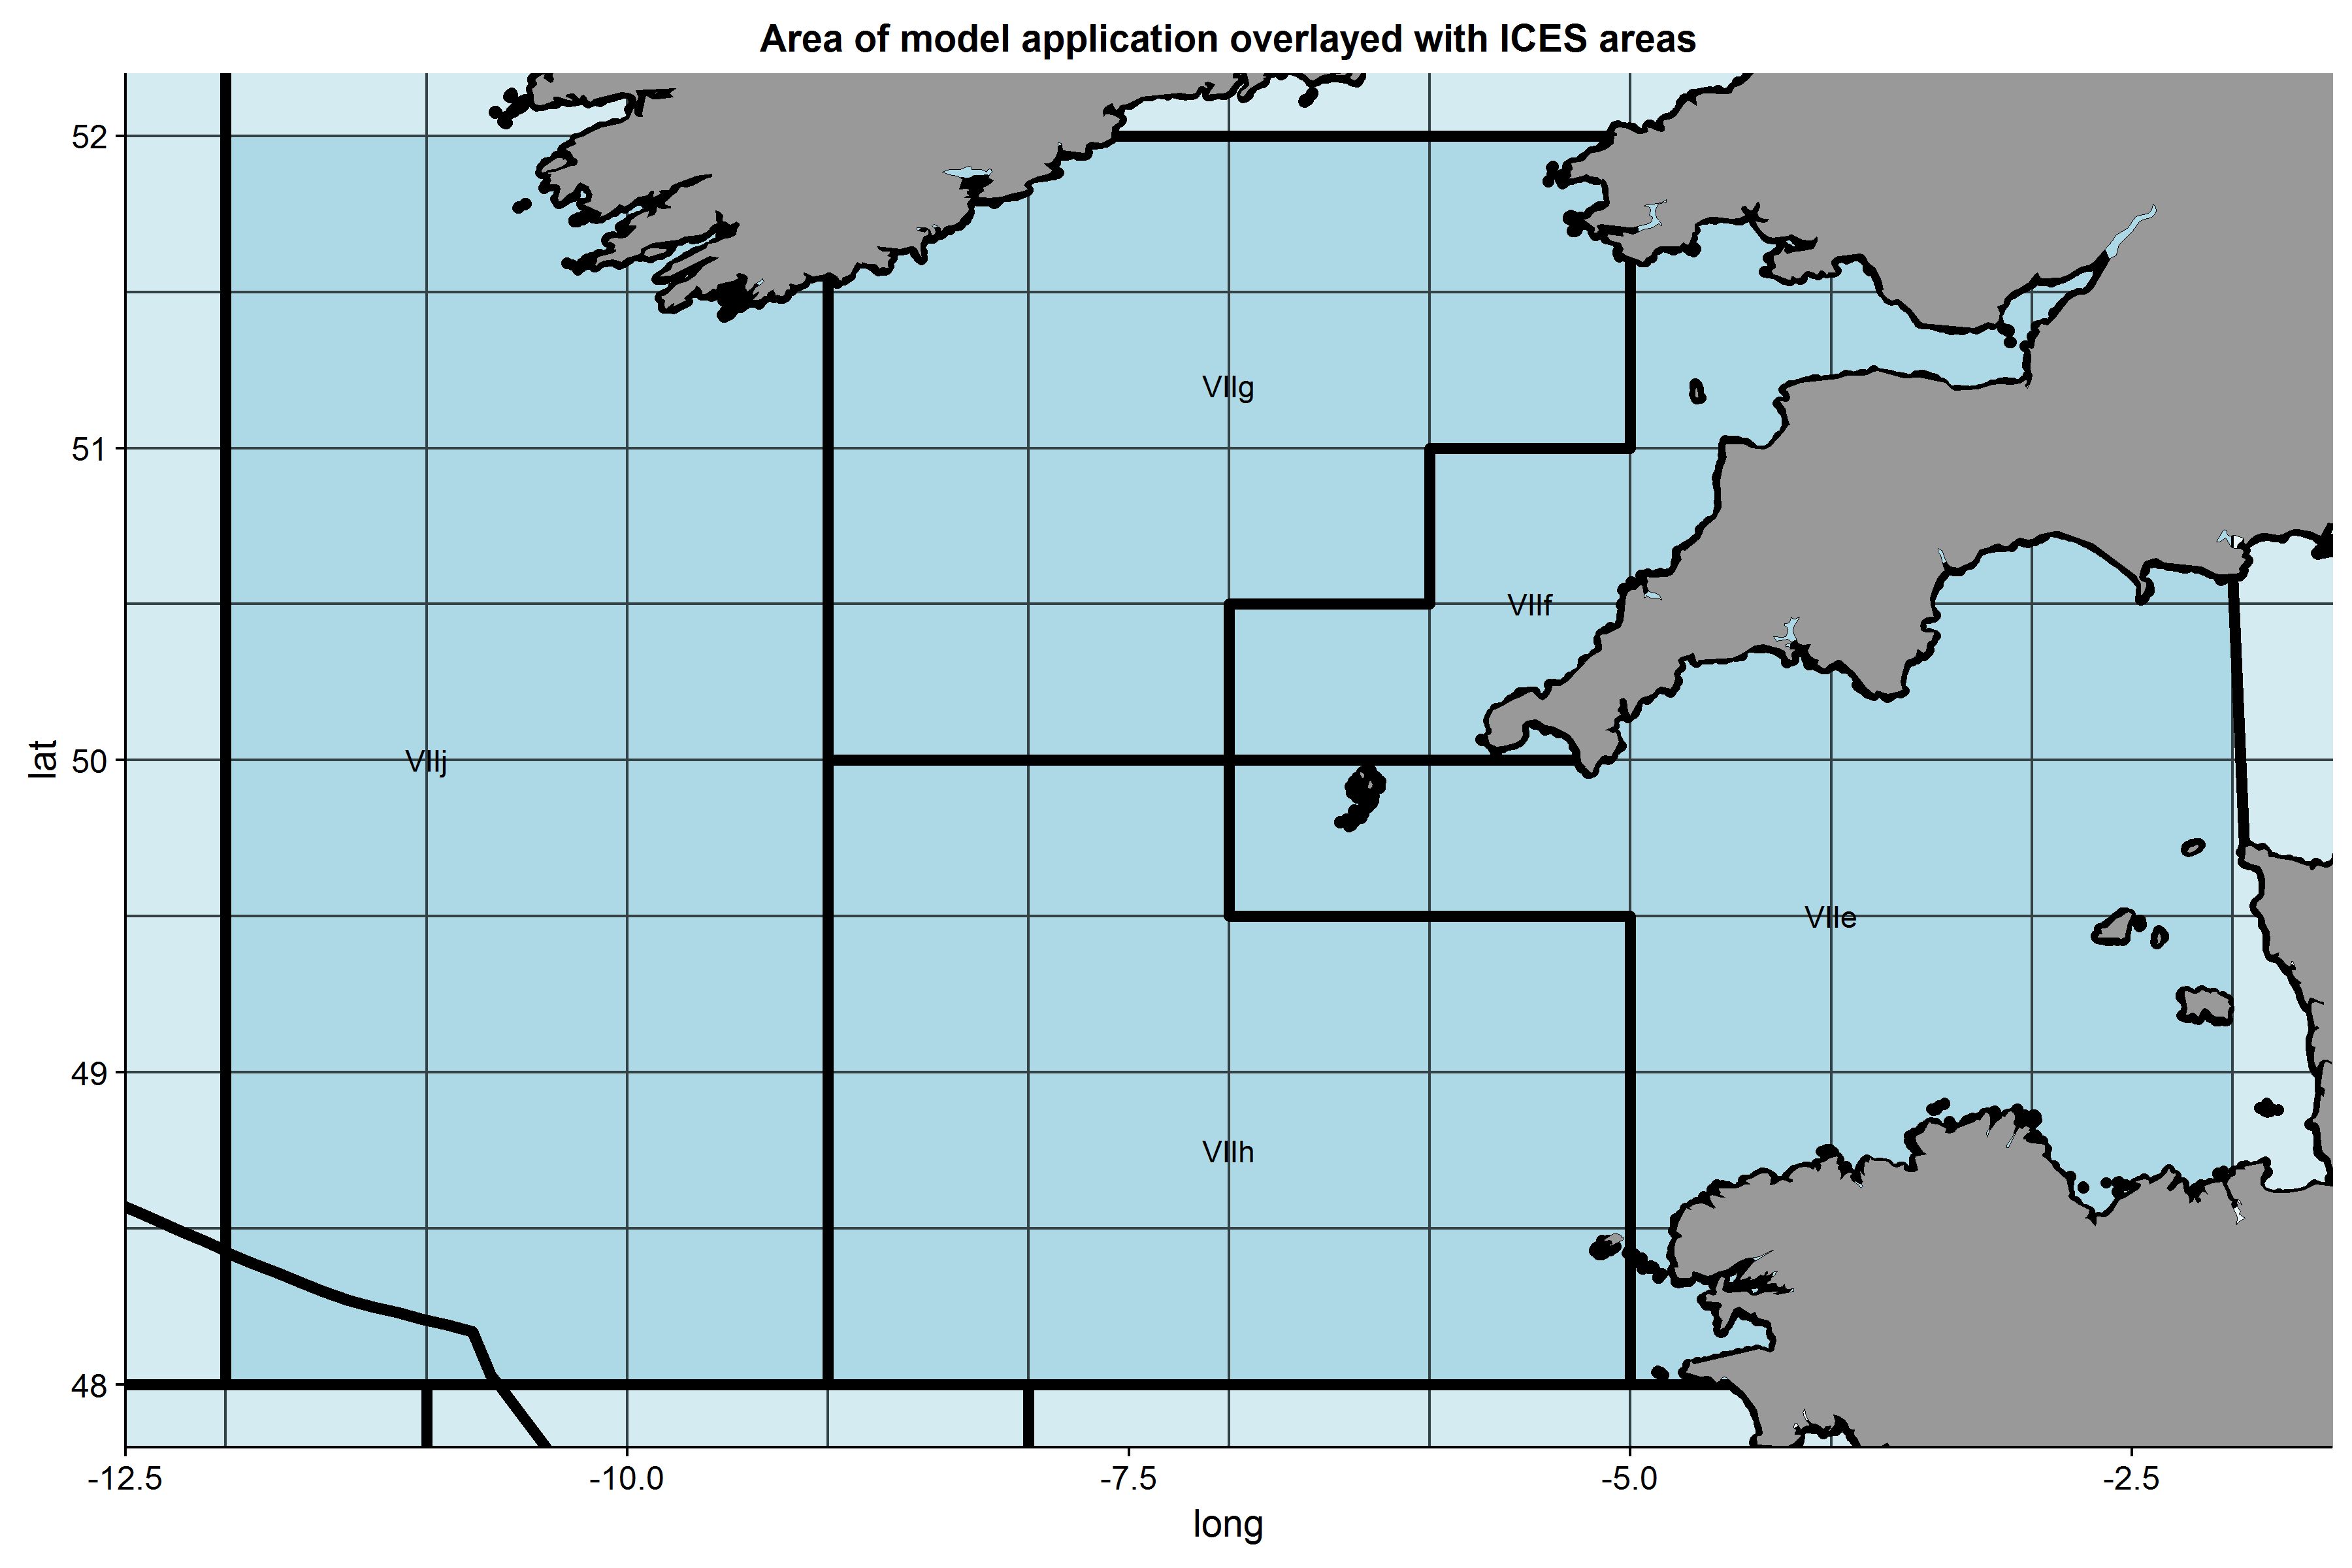
\includegraphics[width=\linewidth]{figure/AreaMap}
\label{fig:1}
\caption{Model was applied to survey data within the dark blue area bound by
	48$^{\circ}$ N to 52 $^{\circ}$ N latitude and 12 $^{\circ}$ W to
	2$^{\circ}$ W longitude.}
\end{figure}

\begin{table}[!htb]
	\caption{List of species codes and names}
	\label{tab:1}
	\center
	\begin{tabular}{ p{3cm} p{4cm} p{5cm} p{2cm}}
		\hline
		Species code & Common name              & Species & MCRS (cm) \\
		\hline
		juv          & Juvenile                 & & \\
		adu          & Adult                    & & \\
		\hline
		bud          & Black bellied anglerfish & \textit{Lophius budgessa} & 32* \\
		cod          & Atlantic cod             & \textit{Gadus morhua} & 35 \\
		had          & Atlatic haddock          & \textit{Melanogrammus	aeglefinus} & 30 \\
		hke          & Atlantic hake            & \textit{Merluccius merluccius} & 27 \\
		meg          & Megrim                   & \textit{Lepidorhombus whiffiagonis} & 20\\
		pisc         & White bellied anglerfish & \textit{Lophius piscatorius} & 32* \\
		ple          & European Plaice          & \textit{Pleuronectes platessa} & 27 \\
		sol          & Common sole              & \textit{Solea solea} & 24 \\
		whg          & Atlantic whiting         & \textit{Merlangius merlangus} & 27 \\
		\hline
		\end{tabular}
		*Monkfish species estimated based on a 500g minimum marketing
		weight

\end{table}

\begin{table}[!htb]
	\caption{List of survey codes, names and brief description}
	\label{tab:2}
	\center
	\begin{tabular}{ p{3cm} p{4cm} p{4cm} p{2cm} }
		\hline
		Survey code    & Name 	& Gear & Temporal extent \\
		\hline
		CEXP / IE-IGFS & Celtic Explorer (IE)   & Otter trawl & 2003 - 2015 \\
		CARLHELMAR     & Carlhelmar (UK)	& Commercial beam trawl & 1989 - 2013 \\
		NWGFS          & North West groundfish survey (UK) & Beam trawl & 1988 - 2015 \\
		Q1SWBEAM       & Quarter 1 south-west beam trawl survey (UK) 	& beam trawl & 2006 - 2015 \\
		Q4SWIBTS       & Quarter 4 south-west international bottom trawl survey (UK) & Otter trawl & 2003 - 2010 \\
		THA2 / EVHOE    & EVHOE survey on Thalasa (FR) & Otter trawl & 1997 - 2015 \\
		WCGFS          & Wstern channel groundfish survey (UK) & Otter
		trawl (Portuguese high headline) & 1982 - 2004 \\
		\hline
	\end{tabular}
\end{table}

The working document briefly outlines the methods used for each of the
components to derive the indices. For a fuller account the reader is encouraged
to review the referenced publications.

%%%%%%%%%%%%%%%%%%%%%%%%%%%%%%%%%%%%%%%%%%%%%%%%%%%%%%%%%%%%%%%%%%%%%%%%%%%%%%%%%%%%%%%%%%%%%
\section{Summary of Methods}

\subsection{Overview}

The modelling framework, VAST, has been developed at the North West Fisheries
Science Center, NOAA to incorporate several methodological developments in
modelling species distributions and deriving standardised abundance indices in
a mixed modelling framework. The following briefly summarises these
developments, though you are encouraged to read the publications listed in the
reference list for further detail. \\ 

\subsection{Modelling framework}

VAST implements a delta-generalised linear mixed modelling (GLMM) framework
that takes account of spatio-temporal correlations among multiple species /
size classes through implementation of a factor analysis.  Spatio-temporal
variation is represented through a three-dimensional Gaussian Random Field,
based on a user-constructed mesh.  \\

To achieve this the model implements several recent advances in geostatistical
analysis of point data. Namely, i) Joint Dynamic Species Distribution Models
(JDSDMs) which are able to take account of latent (unobserved) drivers which
affect species distribution and density for one or more species, ii) separate
modelling of encounter probability and positive catch rates (so called 'delta'
and 'hurdle' models), iii) the use of Gaussian Markov Random Fields (GMRFs) to
model the variation in probability of occurrence and density as a
three-dimensional multivariate process (latitude, longitude and time) while
estimating a spatio-temporal correlation function to capture spatio-temporal
autocorrelation, iv) set in a mixed modelling framework allowing the
incorporation of both systematic (fixed) effects and random effects. \\

The steps involved are briefly summarised as:

\begin{enumerate}
	\item Mesh construction: A spatial grid is constructed based on optimal
		clustering of the available point data using a k-means
		algorithm (in the R package R-INLA \cite{Lindgren2015}). This
		provides \textit{n} knots representing the gaussian random
		fields used to derive spatial encounter probability and density
		estimates.

	\item  Associations among species / species-groups are modelled using
		developments in JDSDMs \cite{Thorson2017}. This involves
		implementing a factor analysis decomposition to define a
		function for each factor that returns a positive or negative
		association of one or more species with any location. Thus
		log-density of any species can then be described as a linear
		combination of factors:
		\begin{equation}
			\theta_{p}(s,t) = \sum_{j=1}^{n_{j}}
			L_{p,j}\psi_{j}(s,t) +\sum_{k=1}^{n_{k}}
			\gamma_{k,p}\chi_{k}(s,t)
		\end{equation}
		Where $\theta_{p}(s,t)$ represents log-density for species $p$
		at site $s$ at time $t$, $\psi_{j}$ is factor $j$, $L_{p,j}$
		the loading matrix representing association of species $p$ with
		factor $j$ and $\gamma_{k,p}\chi_{k}(s,t)$ the linear effect of
		covariates at each site and time \cite{Thorson2016b}. 

		The factor analysis can identify community dynamics and where
		species have similar spatio-temporal patterns, allowing
		inference of species distributions and abundance of poorly
		sampled species through association with other species and
		allows for computation of spatio-temporal correlations among
		species-groups \cite{Thorson2016b}.

	\item Spatio-temporal encounter probability and positive catch rates
		are modelled separately with spatio-temporal encounter
		probability modelled using a logit-link linear predictor;
		\begin{equation}
			logit[p(s_{i},p_{i},t_{i})] = \gamma_{p}(p_{i},t_{i}) +
			\varepsilon_{p}(s_{i},p_{i},t_{i}) + \delta_{p}(p_{i},
			v_{i})
		\end{equation}

		
		and positive catch rates modelling using a gamma- distribution
		\cite{Thorson2015a}.  
		\begin{equation}
			gamma[r(s_{i},p_{i},t_{i})] = \gamma_{p}(p_{i},t_{i}) +
			\varepsilon_{p}(s_{i},p_{i},t_{i}) + \delta_{p}(p_{i},
			v_{i})
		\end{equation}

		With $\gamma_{*}(p_{i},t_{i})$,
		$\varepsilon_{*}(s_{i},p_{i},t_{i})$ and $\delta_{*}(p_{i},
			v_{i})$ representing an intercept, spatio-temporal
			variation and a vessel effect ($v$) respectively for for
			either probability of encounter, $p$ or density $r$.
	
	\item The spatio-temporal variation is modelled using a Gaussian
		Markov Random Field (GMRF) where catch data in nearby locations
		can be correlated, allowing inference about poorly sampled
		locations. A probability distribution for spatio-temporal
		variation in both encounter probability and positive catch rate
		is specified, $\varepsilon_{*}(s,p,t)$, with a
		three-dimensional multivariate normal distribution so that:
		\begin{equation}
			vec[\mathbf{E}_{*}(t)] \sim MVN(0,\mathbf{R}_{*} \otimes
			\mathbf{V}_{{\varepsilon}{*}})
		\end{equation}

		Here, $vec[\mathbf{E}_{*}(t)]$ is the stacked columns of the
		matrices describing $\varepsilon{*}(s,p,t)$ at every location,
		species and time, $\mathbf{R}_{*}$ is a correlation matrix for
		encounter probability or positive catch rates among locations
		and $\mathbf{V}_{*}$ a correlation matrix for encounter
		probability or positive catch rate among species (modelled
		within the factor analysis). $\otimes$ represents the Kronecker
		product so that the correlation among any location and species
		can be computed \cite{Thorson2017}.
		
		Correlations are estimated based on a Matérn covariance
		function where correlation decays smoothly over space/time the
		further from the location sample. This may include geometric
		anisotropy to reflect the fact that correlations may decline in
		one direction faster than another (e.g. moving offshore)
		\cite{Thorson2013}.

	\item A factor analysis can also be undertaken to incorporate
		covariance of vessels as a random effect, or as done here,
		vessel catchability can be estimated as a fixed effect
		$\delta_{s}(v)$ \cite{Thorson2014}. Fixed covariates for
		habitat quality or other predictors of encounter probability /
		density can be incorporated to improve the spatial predictive
		performance \cite{Thorson2017}.

	\item Parameter estimation is undertaken through Laplace approximation
		of the marginal likelihood for fixed effects while integrating
		the joint likelihood (which includes the probability of the
		random effects) with respect to random effects, using Template
		Model Builder (TMB; \cite{Kristensen2015}).

	\item The index of abundance for species $p$ can then be dervied from
		the summation of the spatio-temporal density estimates. 
		\cite{Thorson2017} as: 
		\begin{equation} I(p,t) =
			\sum_{s=1}^{n_{s}} a(s) \cdot
			logit^{-1}[\gamma_{p}(p,t) + \varepsilon_{p}(s,p,t)]
			\cdot exp[\gamma_{r}(p,t) + \varepsilon_{r}(s,p,t)]
		\end{equation}
\end{enumerate}

\subsection{Software}

The software used for the analysis was the R package VAST available on the
authors website (\url{https://github.com/james-thorson/VAST};
\cite{Thorson2017}).  Software version 2.4.0 was used for this analysis. The
package depends on methods in the R-INLA package (\cite{Lindgren2015}) for
defining the spatial fields and Template Model Builder (TMB;
\cite{Kristensen2015}) for maximum likelihood estimation (MLE) of the fixed
effects and integrating across the random effects. \\

Computation was done with support of the Irish Centre for High End Computing
(ICHEC; \url{https://www.ichec.ie}) facility.  \\


\section{Data}

Data were obtained from seven surveys undertaken since 1982 (Table \ref{tab:2};
Figures \ref{fig:d1} and \ref{fig:d2}). For the purpose of this analysis, only
data from stations fished in 1990 - 2015 were used. \\

\begin{figure}[!phtb]
	\centering
\includegraphics[width=0.8\linewidth]{figure/Survey_by_year-1}
\caption{Temporal coverage of the different surveys undertaken in the Celtic
	Sea.* 2016 is incomplete data}
\label{fig:d1}
\end{figure}

\begin{figure}[!phtb]
	\centering
\includegraphics[width=0.8\linewidth]{figure/Survey_effort_by_year-1}
\caption{Number of stations per year for the different surveys undertaken in
	the Celtic Sea.*2016 is incomplete data}
\label{fig:d2}
\end{figure}

See \textbf{Data Annex} for full detail of data processing including code and
summary exploratory plots. \\

In summary:

\begin{itemize}
	\item Station and biological information was either downloaded from
		Datras or obtained directly from Cefas Fishing Survey System
		(FSS).
	\item Data were checked and cleaned for consistency (only valid hauls
		retained, outlier tow duration and distances removed,
		length measurements that were outliers were removed).
	\item Swept area per tow were estimated from the product of distance
		towed,  door spread (estimated through fitting a GAM so that:
		DoorSpread = s(Depth) + DoorWt + WarpLngth + WarpDiam +
		SweepLngth) and a gear and species-type specific correction
		factor.
	\item Length weight conversion factors were estimated from available
		data in Datras (EVHOE survey) and numbers at length were raised
		to weight per length class (based on a split between juveniles
		\textless Minimum Conservation Reference Size (MCRS) and adults
		\textgreater MCRS).
\end{itemize}

\section{Model fitting and choice}

The VAST model was fit to data on nine species in the Celtic Sea (Table
\ref{tab:1}) split into \textgreater MCRS and \textless MCRS (18
species-size-groups in total). The final models were setup as follows:

\begin{itemize}
	\item The data was constrained to 1990 - 2015, reflecting the period
		during which the most spatially consistent data were available.
	\item The GMRF was set to 250 knots (Figure \ref{fig:2}) based on a
		compromise between spatial disaggregation and computational
		efficiency.
	\item The number of factors for the factor analysis decomposition set
		at nine (which explained \textgreater 95 \% of the variance in the
		encounter probability and density).
	\item Distributions
		\begin{itemize}
			\item Encounter probability: Logit-link 
			\item Positive catch rate:   Gamma
		\end{itemize}
	\item Catchability covariates: 108 ((7-1) gears * 18 species) M1,
		M2 only; see Table \ref{tab:3})
	\item Density covariates: 7 substrate categories (defined based on
		EMODnet substrate classification downloaded from
		\url{www.emodnet-seabedhabitats.eu}) and depth as a covariate
		(downloaded from \url{portal.emodnet-bathymetry.eu}) - M2 only
		(see Table \ref{tab:3}).
\end{itemize}

Three models fit:

\begin{table}[!htb]
	\caption{Final three candidate models fit}
	\label{tab:3}
	\center
	\begin{tabular}{ p{3cm} p{4cm} p{4cm} p{2cm} p{2cm} }
		\hline
		Model & Catchability covariates & Density covariates & No Fixed
		effects & No Random effects \\
		\hline
		M0 & Vessel as Random effect & None  & 1462 & 129276 \\
		M1 & Vessel*Species group as fixed effect & None & 1674 & 129276   \\
		M2 & Vessel*Species group as fixed effect & Habitat and depth
		as fixed covariates & 1688 & 129276 \\ 
		\hline
	\end{tabular}
\end{table}

M1 and M2 outperformed M0 based on AIC and BIC, with almost identical AIC
values, indicating little information from including habitat and depth as
covariates.  However, this effect is being explored as a Habitat*Species effect
as further exploration.

\section{Diagnostics}

Figure \ref{fig:2} shows the location of the data (across years) alongside the
knot positions for the gaussian random fields, showing that the locations are
more closely positioned where there are more data points. \\

Figure \ref{fig:3} shows the ordered predicted and observed probability of
encounter for the model fit and Figure \ref{fig:4} shows a Q-Q plot from the
positive catch rates. Both indicate the model has captured the observed
patterns well.

\begin{figure}[!phtb]
	\centering
\includegraphics[width=0.8\linewidth]{figure/SpatialDataAndKnots}
\caption{Locations of data points and the knots determining the spatial mesh}
\label{fig:2}
\end{figure}

\begin{figure}[!phtb]
	\centering
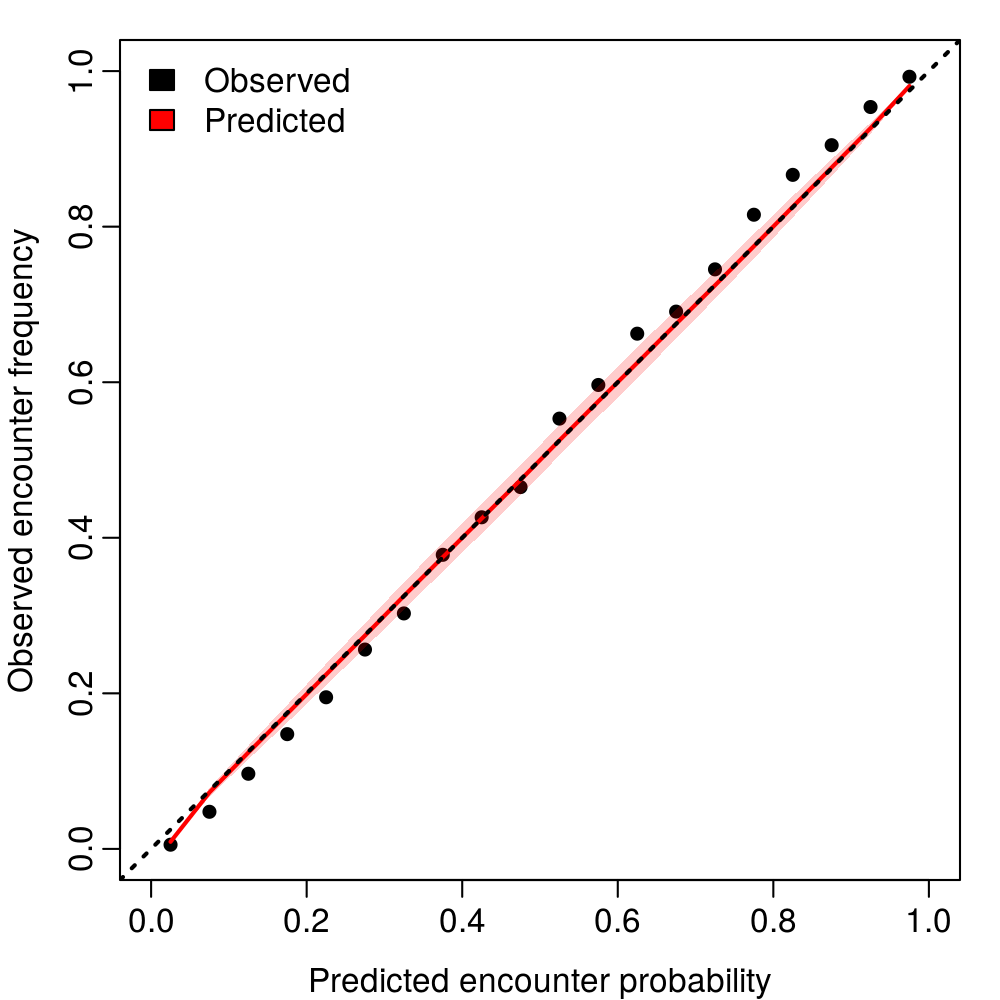
\includegraphics[width=0.6\linewidth]{figure/Diag--Encounter_prob}
\caption{Observed vs predicted encounter probability from the model fit}
\label{fig:3}
\end{figure}

\begin{figure}[!phtb]
	\centering
\includegraphics[width=0.6\linewidth]{figure/Q-Q_plot}
\caption{Q-Q plot for positive catch rate}
\label{fig:4}
\end{figure}

\section{Key outputs}

The following briefly summarises the key figures and outputs from the model
fit. 

\subsection{Catchability covariates}

Figure \ref{fig:5} shows the parameter estimates for the encounter probability
for the different gears (on the x-axis) and species (in panels). Figure
\ref{fig:6} shows the same for positive catch rates. Overall patterns can be
seen where otter trawl surveys tend to be more efficient at catching roundfish
and beam trawl surveys for flatfish, as you would expect. Taking adult cod as
an example (top right panel) the encounter probability for the beam trawl
surveys (3 on the left hand side) are lower than the otter trawl surveys (two
on the right-hand side, and the intercept representing the IE-IGFS), as would
be expected. The interpretation of the catch rate for a survey/species
combination taking account of both encounter probability and positive catch
rate is non-linear due to the logit-link for encounter probability combined
with the log-link for the catch rate.\\

\subsection{Species correlations and factor analysis}

As can be seen in Figure \ref{fig:7} the model estimates stronger geometric
anisotropy in a North East - South West direction with the distance where
correlation decays to 10 \% approximately 100 km. The North West - South East
anisotropy is estimated at approximately half that distance. \\

The average spatial encounter probability factor loadings indicate that 83\% of
the variance can be described by the first three axis loadings. Plotted
spatially there are some indications this is driven by a North East (negatively
associated with factor 1) - South West (positively associated) direction on the
first axis, a North / South division on the second axis and an East / West
split on the third axis (Figure \ref{fig:10}).\\

The spatio-temporal loadings for density on occurrence are less clear from the
factor map (Figure \ref{fig:12}) while the species-group loadings (Figure
\ref{fig:11}) indicate strong association among groups; e.g.  cod, haddock and
whiting \textgreater MCRS are all loaded in the same direction on axis one,
with cod and haddock also loaded in the same direction on axis two, though
whiting is in the opposite direction. \\

The species-group correlations (Figure \ref{fig:8}) show strong positive
associations among intra-species size classes (blocks of four on the diagonal)
for the average spatial encounter probability (top left), spatio-temporal
encounter probability (top right), average density (bottom left) and
spatio-temporal density (bottom right). There are also clear positive
association groupings among the gadoids (cod, haddock, whiting), the flatfish
(plaice and sole) and the deeper water species (anglerfishes, megrim and hake).
\\

\subsection{Global and spatial indices}

Figure \ref{fig:13} presents a global index for each of the species-groups. As
can be seen from Figure \ref{fig:14}, there is good consistency between the
derived indices and the assessment SSB for cod, haddock and whiting despite
there not being total overlap with the size groups (the VAST indices are based
on \textless \hspace{0.1cm} or \hspace{0.1cm} \textgreater \hspace{0.1cm} MCRS
rather than maturity). \\

Figures \ref{fig:15} - \ref{fig:30} display the spatial density estimates for
each of the species groups. As can be seen, the areas with more observations
(tows and therefore closer knots) given a higher resolution from the model. \\

\begin{figure}[!phtb]
	\centering
\includegraphics[width=0.9\linewidth]{figure/QEstimatesGridEnc}
\caption{Estimates of catchability effect on encounter probability. All gear
	effects relative to Celtic Explorer / IE-IGFS}
\label{fig:5}
\end{figure}

\begin{figure}[!phtb]
	\centering
\includegraphics[width=0.9\linewidth]{figure/QEstimatesGridPos}
\caption{Estimates of catchability effect on encounter probability. All gear
	effects relative to Celtic Explorer / IE-IGFS}
\label{fig:6}
\end{figure}

\begin{figure}[!phtb]
	\centering
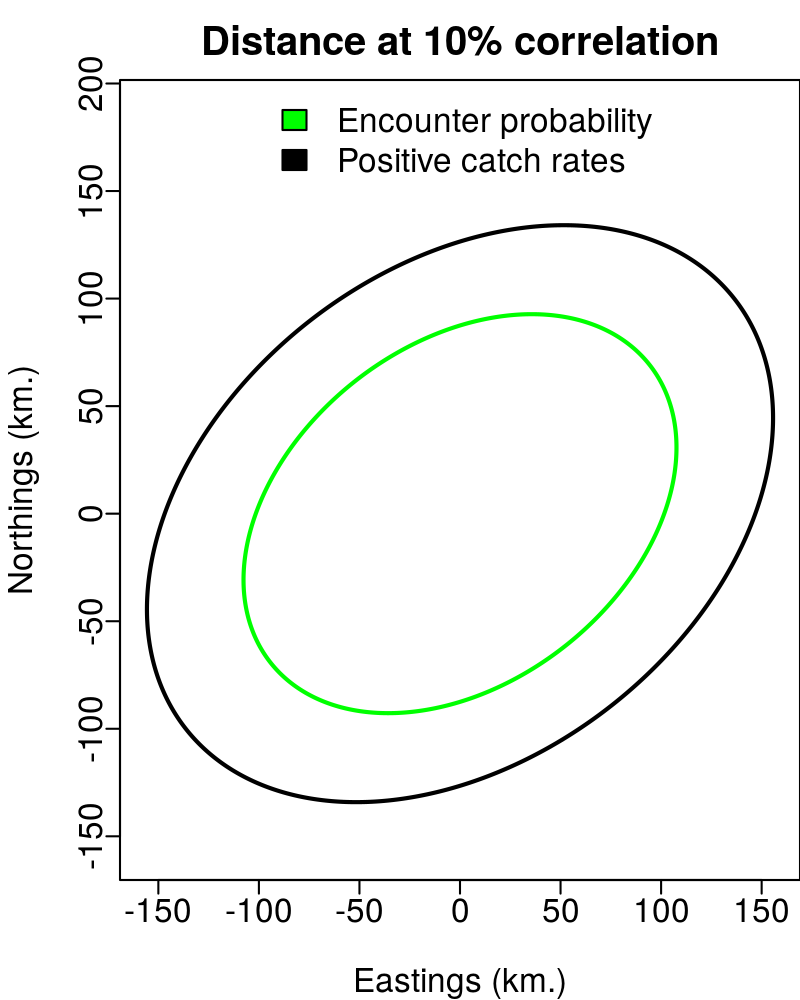
\includegraphics[width=0.5\linewidth]{figure/Aniso}
\caption{Estimates of spatial correlation (Anisotropic effect)}
\label{fig:7}
\end{figure}

\begin{figure}[!phtb]
	\centering
\includegraphics[width=0.9\linewidth]{figure/Factor_loadings--Omega1}
\caption{Factor loadings - average spatial encounter probability}
\label{fig:9}
\end{figure}

\begin{landscape}
\begin{figure}[!phtb]
	\centering
\includegraphics[width=0.9\linewidth]{figure/Factor_maps--Omega1}
\caption{Factor map - average spatial encounter probability}
\label{fig:10}
\end{figure}

\end{landscape}

\begin{figure}[!phtb]
	\centering
\includegraphics[width=0.9\linewidth]{figure/Factor_loadings--Epsilon2}
\caption{Factor loadings - spatio-temporal density}
\label{fig:11}
\end{figure}

\begin{landscape}

\begin{figure}[!phtb]
	\centering
\includegraphics[width=0.9\linewidth]{figure/Factor_maps--Epsilon2}
\caption{Factor map - spatio-temporal density}
\label{fig:12}
\end{figure}

\end{landscape}

\begin{figure}[!phtb]
	\centering
\includegraphics[width=\linewidth]{figure/Spatio-temporal_Covariances--Analytic}
\caption{Species Correlations}
\label{fig:8}
\end{figure}

\begin{landscape}

\begin{figure}[!phtb]
	\centering
\includegraphics[width=0.95\linewidth]{figure/IndexGGplot}
\caption{Global abundance indices}
\label{fig:13}
\end{figure}

\end{landscape}

\begin{figure}[!phtb]
	\centering
\includegraphics[width=0.9\linewidth]{figure/RelativeIndexVRelativeAssessSSB}
\caption{Index relative to assessment}
\label{fig:14}
\end{figure}

%%%%%%%%%%%%%%%%%%%%%%%%%

\begin{landscape}

	%% cod
\begin{figure}[!phtb]
	\centering
\includegraphics[width=\linewidth]{"figure/Field_Dens--Gadus morhua_Adu"}
\caption{Spatial density estimate map - cod adult}
\label{fig:15}
\end{figure}


\begin{figure}[!phtb]
	\centering
\includegraphics[width=\linewidth]{"figure/Field_Dens--Gadus morhua_Juv"}
\caption{Spatial density estimate map - cod juvenile}
\label{fig:16}
\end{figure}

%% haddock
\begin{figure}[!phtb]
	\centering
\includegraphics[width=\linewidth]{"figure/Field_Dens--Melanogrammus aeglefinus_Adu"}
\caption{Spatial density estimate map - haddock adult}
\label{fig:17}
\end{figure}


\begin{figure}[!phtb]
	\centering
\includegraphics[width=\linewidth]{"figure/Field_Dens--Melanogrammus aeglefinus_Juv"}
\caption{Spatial density estimate map - haddock juvenile}
\label{fig:18}
\end{figure}

%% whiting
\begin{figure}[!phtb]
	\centering
\includegraphics[width=\linewidth]{"figure/Field_Dens--Merlangius merlangus_Adu"}
\caption{Spatial density estimate map - whiting adult}
\label{fig:19}
\end{figure}

\begin{figure}[!phtb]
	\centering
\includegraphics[width=\linewidth]{"figure/Field_Dens--Merlangius merlangus_Juv"}
\caption{Spatial density estimate map - whiting juvenile}
\label{fig:20}
\end{figure}

%% pisc 
\begin{figure}[!phtb]
	\centering
\includegraphics[width=\linewidth]{"figure/Field_Dens--Lophius piscatorius_Adu"}
\caption{Spatial density estimate map - Monkfish (piscatorius) adult}
\label{fig:21}
\end{figure}

\begin{figure}[!phtb]
	\centering
\includegraphics[width=\linewidth]{"figure/Field_Dens--Lophius piscatorius_Juv"}
\caption{Spatial density estimate map - Monkfish (piscatorius) juvenile}
\label{fig:22}
\end{figure}

%% bud 
\begin{figure}[!phtb]
	\centering
\includegraphics[width=\linewidth]{"figure/Field_Dens--Lophius budegassa_Adu"}
\caption{Spatial density estimate map - Monkfish (budegassa) adult}
\label{fig:23}
\end{figure}

\begin{figure}[!phtb]
	\centering
\includegraphics[width=\linewidth]{"figure/Field_Dens--Lophius budegassa_Juv"}
\caption{Spatial density estimate map - Monkfish (budegassa) juvenile}
\label{fig:24}
\end{figure}

%% hake
\begin{figure}[!phtb]
	\centering
\includegraphics[width=\linewidth]{"figure/Field_Dens--Merluccius merluccius_Adu"}
\caption{Spatial density estimate map - hake adult}
\label{fig:25}
\end{figure}

\begin{figure}[!phtb]
	\centering
\includegraphics[width=\linewidth]{"figure/Field_Dens--Merluccius merluccius_Juv"}
\caption{Spatial density estimate map - hake juvenile}
\label{fig:26}
\end{figure}


%% plaice
\begin{figure}[!phtb]
	\centering
\includegraphics[width=\linewidth]{"figure/Field_Dens--Pleuronectes platessa_Adu"}
\caption{Spatial density estimate map - plaice adult}
\label{fig:27}
\end{figure}

\begin{figure}[!phtb]
	\centering
\includegraphics[width=\linewidth]{"figure/Field_Dens--Pleuronectes platessa_Juv"}
\caption{Spatial density estimate map - plaice juvenile}
\label{fig:28}
\end{figure}

%% sole  
\begin{figure}[!phtb]
	\centering
\includegraphics[width=\linewidth]{"figure/Field_Dens--Solea solea_Adu"}
\caption{Spatial density estimate map - Sole adult}
\label{fig:29}
\end{figure}

\begin{figure}[!phtb]
	\centering
\includegraphics[width=\linewidth]{"figure/Field_Dens--Solea solea_juv"}
\caption{Spatial density estimate map - Sole juvenile}
\label{fig:30}
\end{figure}


\end{landscape}

\section{Next steps}

The objective for the analysis was to \textbf{i)} Evaluate inter-species
spatio-temporal dynamics of main commercial fish populations in the Celtic Sea
\textbf{ii)} Explore strength of interdependence of fisheries on the different
species (as an insight into the ability to spatially separate catches of
species \textit{x} from species \textit{y}) given they are caught together in
mixed fisheries, and \textbf{iii)} Make efficient use of (and combine) the
various surveys that have been undertaken in the Celtic Sea. \\

VAST provides a fully model-based geo statistical method incorporating spatial
and temporal correlations within and across species and taking account of
differences in survey design. As expected, strong correlations within groups
(gadoids, flats, shelf) indicates may be spatially difficult to separate in
mixed fisheries. \\

The model was fit to data from seven surveys taking place from 1990 - 2015 and
describes well the spatio-temporal dynamics of the 18 species-size-groups
providing insight into their association with each other and spatial
distribution and densities. \\

The derived indices show good agreement with assessment outputs and offer a
potential method to standardise across the various surveys - this may be useful
for producing indices with longer time series than used at present and may be
extended to data poor stocks currently without indices. For this purpise it may
be that data need be at an appropriate age- or size- disaggregation. Another
potential use could be as a useful tool to identify spatial gaps (e.g. look at
SDs of density estimates spatially) or the consequences of removing survey
stations or surveys and what impact that might have on indices.

\section{Acknowledgements}

With thanks to Lisa Readdy (Cefas) for providing an output from the Cefas FSS
database, Colm Lordan, Hans Gerritsen and Dave Stokes (MI) and Ian Holmes,
Stephen Shaw, Tim Earl and Chris Darby (Cefas) for helpful discussions
concerning the data and outputs.

%%%%%%%%%%%%%%%%%%%%%%%%%%%%%%%%%%%%%
\newpage
\bibliographystyle{apalike}
\small{\bibliography{VAST}}

%%%%%%%%%%%%%%%%%%%%%%%%%%%%%%%%%%%%%
\end{document}
%%%%%%%%%%%%%%%%%%%%%%%%%%%%%%%%%%%%%
%%%%%%%%%%%%%%%%%%%%%%%%%%%%%%%%%%%%%
